\begin{figure*}[!ht]
    \centering
    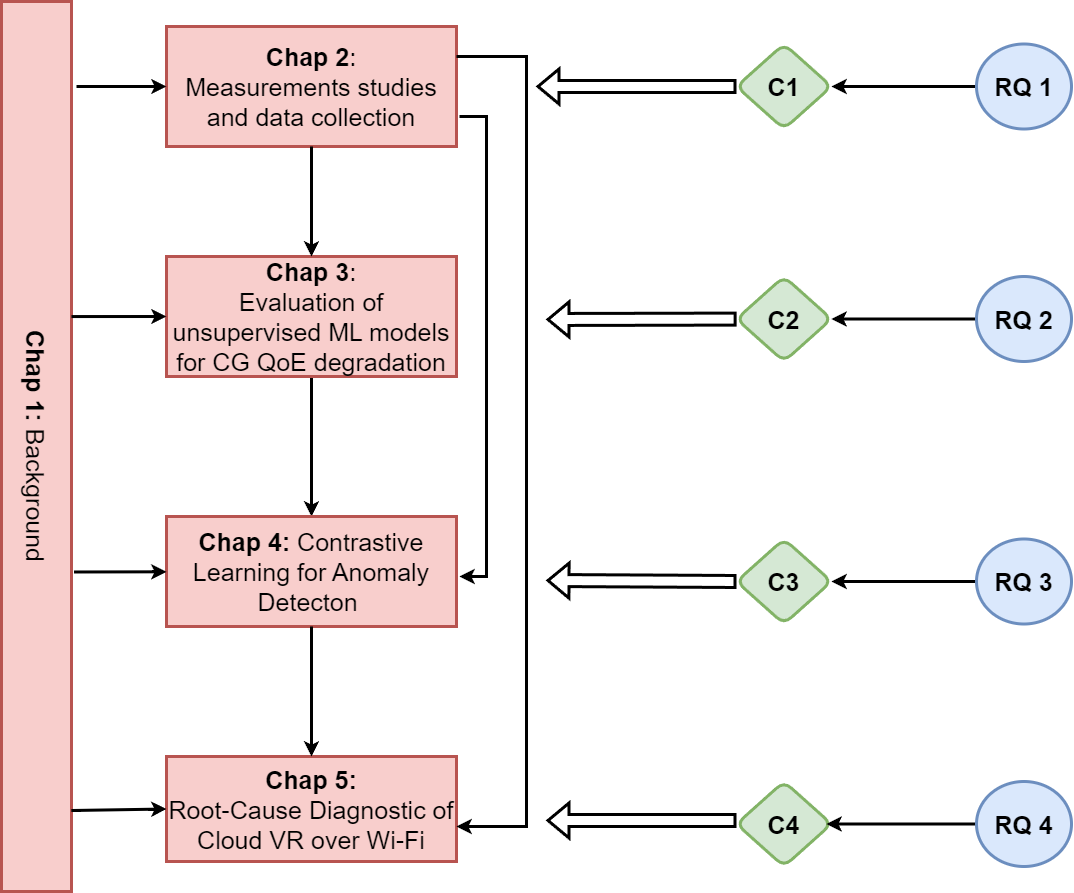
\includegraphics[width=.8\linewidth]{imgs/intro/outline.png}
    \caption{Thesis organization: objectives, contributions and chapters}
    \label{fig:chap_0:thesis_outline}
\end{figure*}


The manuscript is organized into six chapters, introduction and conclusion excluded. The introductory chapter \ref{chap:intro}, outlines the context, goals and motivations behind this thesis and provides a summary of the main contributions. Chapter \ref{chap:related_work} lays the groundwork for the thesis by providing a comprehensive overview of the background and the state of the art in the topics relevant to this research. This includes \ac{LL} applications, cellular and Wi-Fi networks, machine learning, anomaly detection and root-cause diagnosis.

The following chapters detail the research contributions. More specifically, Chapter \ref{chap:measurements} describes the experimental setups and methodologies used to collect datasets in realistic network conditions. Chapter \ref{chap:ml_evaluation} evaluates various unsupervised ML models for anomaly detection in time series using the CG KPIs datasets. 
%Chapter \ref{chap:cg_detection} addresses the problem of CG traffic detection within the scope of the ANR MOSAICO project. It reformulates the detection task as an unsupervised learning task to overcome the generalization limitations of supervised ML models.

In Chapter \ref{chap:cats}, we introduce CATS model for unsupervised anomaly detection in time series using a novel temporal contrastive learning loss function. Building on this, Chapter \ref{chap:diagnosis} proposes a two-stage framework for diagnosis the root causes of performance degradation in Cloud VR applications used over Wi-Fi networks. The manuscript concludes with a synthesis of the findings, highlighting their implications and proposing avenues for future research. A schematic illustration is provided in Fig. \ref{fig:chap_0:thesis_outline}, to clarify how the chapters interconnect, showing the alignment of the research questions with the contributions and the logical progression of the work.



% It explore low-latency applications such as Cloud Gaming and Cloud VR, highlighting the factors influencing user experience. Subsequently, the chapter examines the challenges posed by time-varying capacity network conditions, particularly in cellular and Wi-Fi environments, which can significantly impair low latency applications' performance. Additionally, it introduces machine learning and deep learning frameworks used to tackle anomaly detection and root-cause diagnosis tasks. Finally, the chapter reviews existing approaches for anomaly detection in time series data and root-cause diagnosis techniques in cellular and Wi-Fi networks, identifying key research gaps this research aims to fill.